\documentclass[12pt,a4paper]{article}

\usepackage[utf8]{inputenc}
\usepackage[T1]{fontenc}
\usepackage[brazil]{babel}
\usepackage{times}
\usepackage{geometry}
\usepackage{graphicx}
\usepackage{booktabs}
\usepackage{float}
\usepackage{url}
\usepackage{caption}

\geometry{left=3cm,right=3cm,top=3cm,bottom=2.5cm}
\captionsetup{font=small,labelfont=bf}
\setlength{\parindent}{1.25cm}
\setlength{\parskip}{0pt}

\title{\textbf{Relat\'orio da Atividade 2 -- Etapa 4: Experimentos de Manipula\c{c}\~ao de Mensagens CAN e An\'alise de Impacto}}

\author{
\'Alvaro C. Negromonte\textsuperscript{1},
Victoria Pessoa Barbosa Matos\textsuperscript{1},
Pedro C. Guimar\~aes Rodrigues\textsuperscript{1}
\\[0.3cm]
\textsuperscript{1}Centro de Inform\'atica -- Universidade Federal de Pernambuco (CIn/UFPE)
\\
IF747 -- Redes Automotivas -- 2026.1
\\
Recife -- PE -- Brasil
\\
\texttt{[acn3, vpbm, pcgr]@cin.ufpe.br}
}

\date{}

\begin{document}

\maketitle

\noindent\textbf{Resumo.}
Este relat\'orio apresenta os experimentos de manipula\c{c}\~ao de mensagens CAN
realizados no ambiente Yes, CARLA CAN. Foram executados ataques de \textit{spoofing}
sobre duas fun\c{c}\~oes veiculares, freio de m\~ao e marcha r\'e, al\'em do ataque
\textit{fuzzy}. A an\'alise mostra aumento expressivo na quantidade de mensagens do ID
do freio de m\~ao e evidencia impactos veiculares observados no CARLA, registrados em
v\'ideo durante a execu\c{c}\~ao dos testes.

\section{Introdu\c{c}\~ao}

A Etapa 4 da atividade tem como objetivo manipular mensagens CAN e observar o
impacto dessas altera\c{c}\~oes no comportamento do ve\'iculo simulado. Diferentemente da
etapa de captura e compara\c{c}\~ao geral do tr\'afego, esta etapa enfatiza o efeito funcional
de ataques espec\'ificos sobre fun\c{c}\~oes veiculares.

Foram considerados dois ataques de \textit{spoofing}: um sobre o freio de m\~ao
(\texttt{hand\_brake}) e outro sobre a marcha r\'e (\texttt{reverse}). Tamb\'em foi
executado o ataque \textit{fuzzy}, que injeta mensagens v\'alidas aleat\'orias para
explorar efeitos em diferentes fun\c{c}\~oes veiculares.

\section{Configura\c{c}\~ao Experimental}

Os experimentos foram realizados com o ambiente Yes, CARLA CAN, utilizando o
barramento virtual \texttt{vcan0}. Para esta etapa, foi usado o DBC padr\~ao
\texttt{data/carla.dbc}, pois o m\'odulo de ciberataques define os IDs CAN a partir do
arquivo \texttt{attacks/reverse\_engineering.py}.

O comando de inicializa\c{c}\~ao recomendado para esta etapa \'e:

\begin{verbatim}
./1_up_environment.sh --dbc data/carla.dbc
\end{verbatim}

\section{Ataques Realizados}

\subsection{Spoofing do Freio de M\~ao}

O primeiro ataque foi executado sobre a fun\c{c}\~ao \texttt{hand\_brake}. O alvo foi o ID
CAN \texttt{0x604}, com envio de mensagens peri\'odicas contendo o payload \texttt{01}.
O comando utilizado foi:

\begin{verbatim}
conda run --no-capture-output -n n4s_env python3 cyberattacks_module.py \
  --feature hand_brake --period 0.05
\end{verbatim}

Durante o ataque, observou-se que o ve\'iculo ficou impedido de se mover normalmente,
pois o freio de m\~ao era continuamente for\c{c}ado pelas mensagens injetadas.

Esse impacto foi registrado em v\'ideo. Em compara\c{c}\~ao com o cen\'ario normal, no
qual o ve\'iculo respondia aos comandos de acelera\c{c}\~ao, durante o ataque o ve\'iculo
permanecia parado ou apresentava grande dificuldade para iniciar o deslocamento.

\subsection{Spoofing de Marcha R\'e}

O segundo ataque foi executado sobre a fun\c{c}\~ao \texttt{reverse}. Durante os testes,
foi identificado que o mapeamento original do ataque estava incorreto: o m\'odulo
injetava mensagens no ID \texttt{0x607} com payload \texttt{FF FF FF FF}. No DBC
padr\~ao, entretanto, o ID \texttt{0x607} corresponde \`a mensagem \texttt{GEAR}, enquanto
a mensagem \texttt{REVERSE} corresponde ao ID \texttt{0x603}.

Por isso, o ataque foi corrigido no arquivo \texttt{attacks/reverse\_engineering.py},
alterando o alvo para \texttt{0x603} e o payload para \texttt{01}, compat\'ivel com a
mensagem de 1 byte definida no DBC:

\begin{verbatim}
"reverse": {
    "id": 0x603,
    "payload": [0x01]
}
\end{verbatim}

Ap\'os essa corre\c{c}\~ao, o comando utilizado foi:

\begin{verbatim}
conda run --no-capture-output -n n4s_env python3 cyberattacks_module.py \
  --feature reverse --period 0.05
\end{verbatim}

Com o ID corrigido, o ataque passou a acionar a indica\c{c}\~ao de marcha r\'e no
simulador. Esse resultado confirma que o problema observado inicialmente n\~ao estava
na recep\c{c}\~ao do CARLA, mas sim no ID CAN usado pelo m\'odulo de ataque.

\subsection{Ataque Fuzzy}

O ataque \textit{fuzzy} foi executado com o comando:

\begin{verbatim}
conda run --no-capture-output -n n4s_env python3 cyberattacks_module.py \
  --feature fuzzy --period 0.05
\end{verbatim}

Na implementa\c{c}\~ao atual do reposit\'orio, o argumento \texttt{--period} n\~ao controla
o intervalo real do \textit{fuzzy}; o c\'odigo escolhe fun\c{c}\~oes aleat\'orias e envia
mensagens em intervalos aleat\'orios entre 0,5 s e 1,0 s. Durante sua execu\c{c}\~ao,
foram observados efeitos visuais no simulador. Os efeitos mais f\'aceis de perceber foram
a abertura das portas e o acionamento do freio de m\~ao. Outros efeitos podem ocorrer,
mas s\~ao mais r\'apidos ou menos evidentes visualmente, pois as mensagens normais do
ve\'iculo podem sobrescrever rapidamente parte das mensagens injetadas.

\section{Resultados Quantitativos}

A Tabela~\ref{tab:ataques} resume os ataques executados e seus efeitos observados.

\begin{table}[H]
\centering
\caption{Resumo dos ataques executados na Etapa 4.}
\label{tab:ataques}
\begin{tabular}{llll}
\toprule
\textbf{Ataque} & \textbf{ID CAN} & \textbf{Per\'iodo} & \textbf{Efeito observado} \\
\midrule
hand\_brake & \texttt{0x604} & 0,05 s & Freio de m\~ao for\c{c}ado \\
reverse & \texttt{0x603} & 0,05 s & Indicador de marcha r\'e acionado \\
fuzzy & vari\'avel & aleat\'orio & Portas e freio de m\~ao percept\'iveis \\
\bottomrule
\end{tabular}
\end{table}

Para o ataque \texttt{hand\_brake}, tamb\'em foi realizada an\'alise quantitativa do
tr\'afego CAN. A contagem do ID \texttt{0x604} aumentou de 342 mensagens no cen\'ario
normal para 2003 mensagens durante o ataque, totalizando 1661 mensagens adicionais.
A taxa do ID atacado passou de aproximadamente 4,82 mensagens/s para 22,78
mensagens/s.

\begin{figure}[H]
\centering
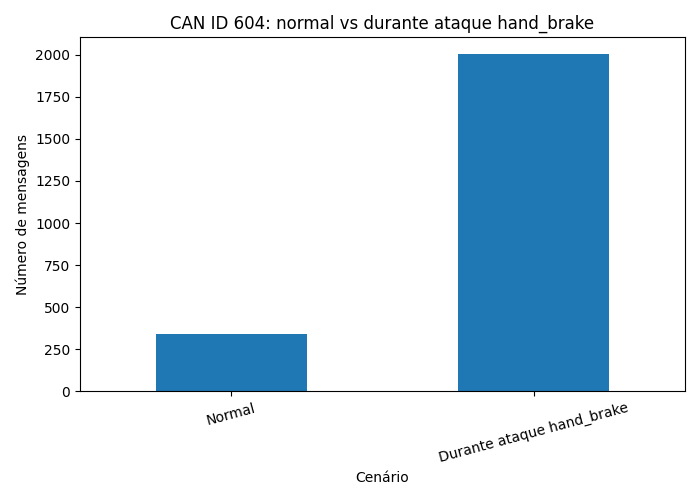
\includegraphics[width=0.86\linewidth]{figures/contagem_id_604_handbrake.png}
\caption{Contagem do ID \texttt{0x604} no cen\'ario normal e durante o ataque \texttt{hand\_brake}.}
\label{fig:count-604}
\end{figure}

\begin{figure}[H]
\centering
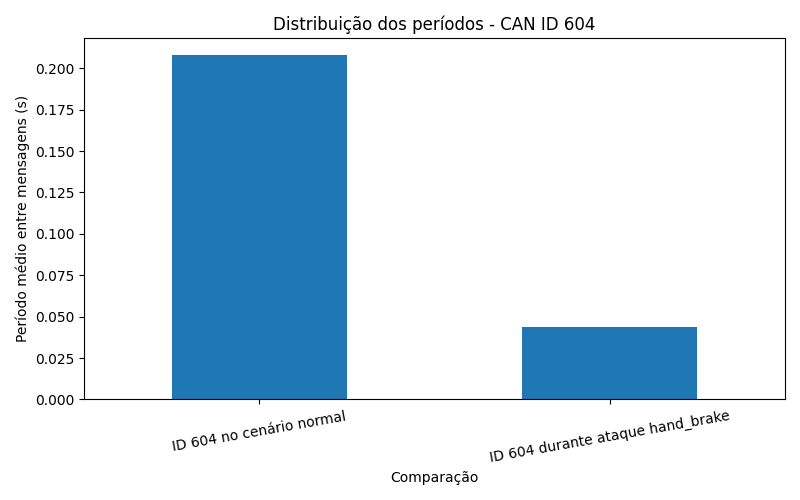
\includegraphics[width=0.86\linewidth]{figures/periodo_id_604.png}
\caption{Per\'iodo m\'edio do ID \texttt{0x604} antes e durante o ataque \texttt{hand\_brake}.}
\label{fig:period-604}
\end{figure}

\section{Discuss\~ao}

Os resultados mostram que os ataques de \textit{spoofing} alteraram diretamente o
padr\~ao temporal dos IDs atacados quando as mensagens s\~ao injetadas com o ID e o
payload corretos. O ID \texttt{0x604}, associado ao freio de m\~ao, passou a aparecer com
frequ\^encia muito maior durante o ataque, o que explica o impacto observado no
simulador: o ve\'iculo n\~ao conseguia se deslocar normalmente.

O caso do \texttt{reverse} tamb\'em mostra a import\^ancia do DBC na interpreta\c{c}\~ao das
mensagens. Antes da corre\c{c}\~ao, o ataque enviava mensagens para \texttt{0x607}, mas
esse ID era decodificado como \texttt{GEAR}. Por isso, o campo visual de marcha r\'e n\~ao
era acionado. Ap\'os alterar o ataque para \texttt{0x603\#01}, o receptor passou a
interpretar corretamente a mensagem como \texttt{REVERSE}.

No ataque \textit{fuzzy}, os efeitos observados foram intermitentes, como esperado,
pois a fun\c{c}\~ao atacada \'e escolhida aleatoriamente. Mesmo assim, foi poss\'ivel notar
impactos visuais claros quando as mensagens sorteadas afetavam portas ou freio de m\~ao,
que s\~ao fun\c{c}\~oes de percep\c{c}\~ao imediata no simulador.

Esse comportamento evidencia uma fragilidade do protocolo CAN: os receptores
interpretam mensagens com base no ID e no formato esperado, mas o protocolo n\~ao
oferece autentica\c{c}\~ao nativa da origem da mensagem. Assim, uma mensagem falsa mas
bem formatada pode ser aceita como leg\'itima pela rede.

\section{Conclus\~ao}

A Etapa 4 demonstrou que ataques de \textit{spoofing} podem causar impacto funcional
vis\'ivel no ve\'iculo simulado e, ao mesmo tempo, gerar altera\c{c}\~oes mensur\'aveis no
tr\'afego CAN. O ataque sobre \texttt{hand\_brake} aumentou expressivamente a contagem
do ID \texttt{0x604} e impediu o deslocamento normal do ve\'iculo. O ataque
\texttt{reverse}, inicialmente incompat\'ivel com o DBC por usar o ID de \texttt{GEAR},
passou a funcionar ap\'os a corre\c{c}\~ao para o ID \texttt{0x603}. O ataque
\textit{fuzzy} tamb\'em produziu efeitos observ\'aveis, principalmente abertura de portas
e acionamento do freio de m\~ao.

Os testes foram registrados em v\'ideo para documentar a diferen\c{c}a de comportamento
do ve\'iculo com e sem os ataques em execu\c{c}\~ao. Os resultados evidenciam que a
inje\c{c}\~ao de mensagens CAN bem formatadas pode alterar fun\c{c}\~oes veiculares no
simulador, refor\c{c}ando a import\^ancia de mecanismos de autentica\c{c}\~ao, valida\c{c}\~ao
e detec\c{c}\~ao de intrus\~oes em redes automotivas.

\end{document}
